% Options for packages loaded elsewhere
\PassOptionsToPackage{unicode}{hyperref}
\PassOptionsToPackage{hyphens}{url}
\PassOptionsToPackage{dvipsnames,svgnames,x11names}{xcolor}
%
\documentclass[
  12pt,
]{article}
\usepackage{amsmath,amssymb}
\usepackage{lmodern}
\usepackage{iftex}
\ifPDFTeX
  \usepackage[T1]{fontenc}
  \usepackage[utf8]{inputenc}
  \usepackage{textcomp} % provide euro and other symbols
\else % if luatex or xetex
  \usepackage{unicode-math}
  \defaultfontfeatures{Scale=MatchLowercase}
  \defaultfontfeatures[\rmfamily]{Ligatures=TeX,Scale=1}
\fi
% Use upquote if available, for straight quotes in verbatim environments
\IfFileExists{upquote.sty}{\usepackage{upquote}}{}
\IfFileExists{microtype.sty}{% use microtype if available
  \usepackage[]{microtype}
  \UseMicrotypeSet[protrusion]{basicmath} % disable protrusion for tt fonts
}{}
\makeatletter
\@ifundefined{KOMAClassName}{% if non-KOMA class
  \IfFileExists{parskip.sty}{%
    \usepackage{parskip}
  }{% else
    \setlength{\parindent}{0pt}
    \setlength{\parskip}{6pt plus 2pt minus 1pt}}
}{% if KOMA class
  \KOMAoptions{parskip=half}}
\makeatother
\usepackage{xcolor}
\usepackage[margin=1in]{geometry}
\usepackage{longtable,booktabs,array}
\usepackage{calc} % for calculating minipage widths
% Correct order of tables after \paragraph or \subparagraph
\usepackage{etoolbox}
\makeatletter
\patchcmd\longtable{\par}{\if@noskipsec\mbox{}\fi\par}{}{}
\makeatother
% Allow footnotes in longtable head/foot
\IfFileExists{footnotehyper.sty}{\usepackage{footnotehyper}}{\usepackage{footnote}}
\makesavenoteenv{longtable}
\usepackage{graphicx}
\makeatletter
\def\maxwidth{\ifdim\Gin@nat@width>\linewidth\linewidth\else\Gin@nat@width\fi}
\def\maxheight{\ifdim\Gin@nat@height>\textheight\textheight\else\Gin@nat@height\fi}
\makeatother
% Scale images if necessary, so that they will not overflow the page
% margins by default, and it is still possible to overwrite the defaults
% using explicit options in \includegraphics[width, height, ...]{}
\setkeys{Gin}{width=\maxwidth,height=\maxheight,keepaspectratio}
% Set default figure placement to htbp
\makeatletter
\def\fps@figure{htbp}
\makeatother
\setlength{\emergencystretch}{3em} % prevent overfull lines
\providecommand{\tightlist}{%
  \setlength{\itemsep}{0pt}\setlength{\parskip}{0pt}}
\setcounter{secnumdepth}{5}
\newlength{\cslhangindent}
\setlength{\cslhangindent}{1.5em}
\newlength{\csllabelwidth}
\setlength{\csllabelwidth}{3em}
\newlength{\cslentryspacingunit} % times entry-spacing
\setlength{\cslentryspacingunit}{\parskip}
\newenvironment{CSLReferences}[2] % #1 hanging-ident, #2 entry spacing
 {% don't indent paragraphs
  \setlength{\parindent}{0pt}
  % turn on hanging indent if param 1 is 1
  \ifodd #1
  \let\oldpar\par
  \def\par{\hangindent=\cslhangindent\oldpar}
  \fi
  % set entry spacing
  \setlength{\parskip}{#2\cslentryspacingunit}
 }%
 {}
\usepackage{calc}
\newcommand{\CSLBlock}[1]{#1\hfill\break}
\newcommand{\CSLLeftMargin}[1]{\parbox[t]{\csllabelwidth}{#1}}
\newcommand{\CSLRightInline}[1]{\parbox[t]{\linewidth - \csllabelwidth}{#1}\break}
\newcommand{\CSLIndent}[1]{\hspace{\cslhangindent}#1}
\usepackage{polyglossia}
\setmainlanguage{turkish}
\usepackage{booktabs}
\usepackage{caption}
\captionsetup[table]{skip=10pt}
\ifLuaTeX
  \usepackage{selnolig}  % disable illegal ligatures
\fi
\IfFileExists{bookmark.sty}{\usepackage{bookmark}}{\usepackage{hyperref}}
\IfFileExists{xurl.sty}{\usepackage{xurl}}{} % add URL line breaks if available
\urlstyle{same} % disable monospaced font for URLs
\hypersetup{
  pdftitle={TÜrkiye'de Yıllara ve İllere Göre Evlenme Sayıları},
  pdfauthor={Fatih YARAR},
  colorlinks=true,
  linkcolor={Maroon},
  filecolor={Maroon},
  citecolor={Blue},
  urlcolor={blue},
  pdfcreator={LaTeX via pandoc}}

\title{TÜrkiye'de Yıllara ve İllere Göre Evlenme Sayıları}
\author{Fatih YARAR\footnote{21080154, \href{https://github.com/fatihyrr/final}{Github Repo}}}
\date{}

\begin{document}
\maketitle
\begin{abstract}
Türkiye, aile kültürünün en güzel yaşandığı ülkelerden biridir. Daha çok gelenekçi bir aile yapısı mevcuttur. Ancak son yıllarda baktığımızda ülkemizde aile yapısının giderek dönüşüme uğradığı görülmektedir. Kültürel değişim, sosyo-ekonomik gelişme, bireysel tutumlar, modernleşme gibi birçok neden, aile ve evlilik kavramlarına bakış açımızın değişmesine neden olmuştur .Değişen bu bakış açısı hem ailenin önemi giderek azaltmış hem insanlarda evlenmenin önüne bir engel olarak çıkmıştır. Evlenme yaşı da oldukça yükselmeye başlamış ve doğurganlık oranında düşmesine yol açmıştır . Kadınlar evlenme olayında artık önemli bir faktör haline gelmiş kendi karar mekanizmasına sahip bireyler olmuşlardır ve toplumda kadının önemi artmıştır. Kadınların da eğitim ve iş hayatına atılmalarıyla birlikte evlenme için karar ailelerden bir nevi bireylere geçmiştir. Türkiye devam eden ekonomik kriz, boşanmaların artması evlenme oranlarının düşlemesine neden olmuştur
\end{abstract}

\hypertarget{giriux15f}{%
\section{Giriş}\label{giriux15f}}

Türkiye nüfusunun çoğunluğu evlilik kurumuna önem veren bir topluluktur.Türk kültüründe toplumun temel yapı taşlarından biridir ve genellikle sosyal bağların kuvvetlendirildiği bir araçtır. Ancak son yıllara baktığımızda Türkiye'de evlilik yaşının yükseldiği de aşikardır Türkiye'de evlilik yaşının yükselmesi ve evliliklerin ertelenmesi eğilimi görülmektedir. Türkiye genç bir nüfusa sahip bir ülkedir, bu genç nüfusun eğitimine ve kariyer hedeflerine daha fazla odaklanmasından kaynaklanmaktadır. Kadınlarında işgücü katılımının artması evlilik yaşının yükselmesine sebep olan etkenlerden biridir.Türkiye'de evlilik sayıları yıllara göre değişiklik göstermektedir. Bu değişiklikler çeşitli faktörlerden etkilenebilir, örneğin ekonomik durum, eğitim seviyesi, kadınların işgücüne katılımı, kültürel değişimler ve demografik faktörler gibi etmenler rol oynayabilir.(Çobanoğlu ve Serhat (\protect\hyperlink{ref-ccobanouglu2021turkiye}{2021})) Ankara, İstanbul, İzmir gibi büyükşehirlere baktığımızda evlilik sayılarının nüfusa oranla bir azalma olduğunu görmekteyiz buralarda nüfus artarken evlenme sayıları hemen hemen aynı kalmıştır. Diğer yandan Türkiye'nin doğu kesime baktığımızda genel olarak orada da evlilik sayılarının arttığını görmekteyiz. Bunun sebepleri olarak da o bölgede doğurganlığın fazla olması (bir çiftin 5,6 çocuğunun olması) gibi etkenler sayılabilir. Bunlara ek olarak insanlar değişen dünyaya ayak uydurarak nikahsız yaşamaya başlaması, artan ekonomik problemler yüzünden evlenmeden sevgili ve flört şeklinde yaşaması bu sayılarda değişkenlik yaşanmasına sebep olmuştur. Ben bu çalışmamda TÜİK'İN YAYINLADIĞI 2009-2022 YILLARI ARASINDATÜRKİYE'DE İLLERE GÖRE EVLİLİK SAYILARI VERİ SETİNİ kullanarak evlilik sayısında yaşanan değişimleri gözlemleyip analiz edeceğim.

\hypertarget{uxe7alux131ux15fmanux131n-amacux131}{%
\subsection{Çalışmanın Amacı}\label{uxe7alux131ux15fmanux131n-amacux131}}

2009 -2022 yılları arasında Türkiyede iller göre evlenme sayılarının göre değişimlerini analiz edebilmeyi konu edinmiştir.
Türkiye son 13 yılda illere evlenme sayılarının hangi yönde ilerlediği, Bireysel gibi görünse de evlenme sayılarının toplumsal olaylardan etkilenip etkilenmediğini ,etkilendiyse nasıl etkilendiğini istatistiksel yöntemlere başvurarak ,sosyodemografik açıdan incelemeyi ve sebeplerini kaynaklar ve veriler doğrultusunda istatiksel analiz yapabilmeyi amaçlanmaktadır .

\hypertarget{literatuxfcr}{%
\subsection{Literatür}\label{literatuxfcr}}

Toplumun en küçük birimi olarak kabul edilen aile, bireyin en temel sosyal çevresini oluşturmaktadır (Özgüven, 2014, 1). Aile kurumunun varlığı ve sürekliliği evlilik aracılığıyla sağlanmaktadır. Evlilik ise, kadın ve erkek ilişkisini meşru bir temele dayandıran toplumsal olgudur (Doğan, 2007, 208). Özgüven'e (2014, 19) göre ise evlilik, karşı cinsten iki kişinin birlikte yaşama, çocuk yapma ve yetiştirme, deneyimleri paylaşma gibi amaçlar ile yaptıkları bir sözleşmedir. Evlilik, devlet tarafından birtakım yasa ve düzenlemeler ile kontrol edilen yasal bir ilişkidir.(İlhan ve Işık (\protect\hyperlink{ref-ilhan2019marriage}{2019}))Türkiye'de yaşanan demografik dönüşüm, kentleşme, eğitimin yaygınlaşması, gelirin artması, yaşam ve tüketim tarzlarında farklılaşma gibi toplumsal dönüşüm süreçlerine bağlı olarak erken evliliklerin yaygınlığı giderek azalmaktadır. Modernleşme ile birlikte toplumlarda aile kurumunun dönüşümüne neden olan çok sayıda süreç aynı anda yaşanmaktadır.Son yıllarda gençlerin evlilik yaşının yükseldiği ve evlilik öncesi ilişkilerin süresinin uzadığı gözlemlenmektedir.(BAKANLIĞI ve MÜDÜRLÜĞÜ (\protect\hyperlink{ref-bakanliugi2015turkiye}{2015})). Nüfusu ve haneyi ilgilendiren konulardan biri de evlilik yaşıdır. Türkiye'de evlilik yaşı son yıllarda giderek yükselmektedir2000 yılında Türkiye'de kadınlarda ilk evlenme yaşı ortalaması 23,2'den 2015 yılında 23.9'a yükselmiştir.Türkiye'de evliliklerin çoğunluğu . Özellikle kırsal bölgelerde ve daha muhafazakar toplumlarda, genç yaşta evlenme yaygındır. TÜİK'in tespitine göre Ağrı'da 2015 yılında kadınların ortalama evlenme yaşı 21.2'dir.(KOÇ vd. (\protect\hyperlink{ref-kocc2017development}{2017}),)Türkiye'de boşanma oranlarının da arttığı görülmektedir. Çiftler arasındaki uyumsuzluklar, iletişim sorunları, ekonomik zorluklar, aile baskısı ve diğer faktörler boşanmalara neden olabilir. Boşanma oranları, kentsel bölgelerde ve daha eğitimli kesimlerde genellikle daha yüksek olma eğilimindedir.Bu yüzdende insanlar erken yaşta evlenmeyi değil nikahsız bir birliktelik yada dini nikahlı bir birliktelik yaşamaktadırlar.Cinsiyet ayrımcılığına karşı çıkan mücadeleler sonucunda batı toplumlarında cinsiyetler arasında büyük oranda siyasal, ekonomik ve toplumsal eşitlik sağlanmıştır. Bu süreç sonunda kadının toplumsal yapı içerisinde edilgen bir yapıdan etkin bir konuma geçmesiyle; evlenme ve boşanma gibi sosyal olgularda modern yaşama özgü yeni durumlar ortaya çıkmıştır.((\protect\hyperlink{ref-aydin2010toplumsal}{\textbf{aydin2010toplumsal?}}))

\hypertarget{veri}{%
\section{Veri}\label{veri}}

Bu çalışmam kullandığım veri TÜİK'in yayımlamış olduğu veriler içerisinden seçmiş olduğum 2002-2022 yılları arasında İllere Göre EVlenme oranları adlı veri setidir.BU veriyi aldıktan sonra üzerinde bir takım değişikliklerde bulundum.Normalde 21 değişken bulunmaktaydı.Ben bu değişkelerin sayısı fazla olduğu için ilk 7 yıllık verisini silerek 14 değişkene düşürmüş oldum .83 olan gözlem sayısını ise 82'ye düşürüp ortaya çıkabilecek karmaşık tabloların ve grafiklerin önüne geçmiş oldum

Evlilik Sayıları: Evlilik sayıları yıl yıl değişmektedir. Ortalama değerlere bakarak, yıllar arasındaki evlilik sayılarının genel bir trende sahip olduğunu gözlemleyebiliriz. Örneğin, en yüksek ortalama evlilik sayısı 2009 yılında 7305.46 iken, en düşük ortalama evlilik sayısı 2020 yılında 6028.83 olarak görülmektedir.

Dağılım: Evlilik sayılarının standart sapma değerleri, yıllar arasındaki değişkenliği gösterir. Yüksek standart sapma değerleri, evlilik sayılarının yıllar arasında büyük ölçüde değiştiğini ve dağılımın geniş olduğunu gösterir. Örneğin, 2009 yılındaki standart sapma 12117.10 iken, 2016 yılındaki standart spma 10541.60 olarak görülmektedir.

Medyan Evlilik Sayısı: Medyan değeri, evlilik sayılarının orta noktasını gösterir. Medyan değeri, evlilik sayılarının dağılımında daha az etkilenen bir ölçüdür. Örneğin, 2011 yılında medyan evlilik sayısı 4048 iken, 2019 yılında 3479 olarak görülmektedir.

En Yüksek ve En Düşük Evlilik Sayısı: Tablodaki verilere göre, yıllar arasında en yüksek ve en düşük evlilik sayıları değişmektedir. Örneğin, en yüksek evlilik sayısı 2011 yılında 114382 iken, en düşük evlilik sayısı 2020 yılında 3046 olarak görülmektedir.

\begin{table}[ht]
\centering
\caption{Özet İstatistikler} 
\label{tab:ozet}
\begin{tabular}{lccccc}
  \toprule
 & Ortalama & Std.Sap & Min & Medyan & Mak \\ 
  \midrule
ikibindokuz & 7305.46 & 12117.10 & 599.00 & 4338.00 & 100406.00 \\ 
  ikibinon & 7194.01 & 12490.42 & 604.00 & 4043.00 & 104055.00 \\ 
  ikibinonaltı & 7339.42 & 13600.66 & 465.00 & 3648.00 & 113059.00 \\ 
  ikibinonbeş & 7444.22 & 13748.38 & 495.00 & 3875.00 & 114382.00 \\ 
  ikibinonbir & 7318.21 & 12775.04 & 574.00 & 4048.00 & 105860.00 \\ 
  ikibinondokuz & 6695.23 & 12095.45 & 428.00 & 3479.00 & 100088.00 \\ 
  ikibinondört & 7403.75 & 13468.51 & 528.00 & 3995.00 & 112141.00 \\ 
  ikibinoniki & 7453.72 & 13293.73 & 547.00 & 4020.00 & 110478.00 \\ 
  ikibinonsekiz & 6844.31 & 12270.33 & 403.00 & 3490.00 & 101333.00 \\ 
  ikibinonüç & 7409.11 & 13344.35 & 528.00 & 4098.00 & 111050.00 \\ 
  ikibinonyedi & 7030.36 & 12813.59 & 445.00 & 3596.00 & 106053.00 \\ 
  ikibinyirmi & 6028.83 & 10541.60 & 355.00 & 3046.00 & 86029.00 \\ 
  ikibinyirmibir & 6952.35 & 12092.73 & 429.00 & 3547.00 & 98796.00 \\ 
  ikibinyirmiiki & 7090.84 & 12856.82 & 394.00 & 3552.00 & 105694.00 \\ 
   \bottomrule
\end{tabular}
\end{table}

\hypertarget{a-tibble-81-x-14}{%
\section{A tibble: 81 x 14}\label{a-tibble-81-x-14}}

ikibinonbir ikibind\textasciitilde1 ikibi\textasciitilde2 ikibi\textasciitilde3 ikibi\textasciitilde4 ikibi\textasciitilde5 ikibi\textasciitilde6 ikibi\textasciitilde7 ikibi\textasciitilde8
1 574 638 604 596 528 566 513 470 445
2 608 599 605 547 547 528 495 465 460
3 894 887 932 893 831 761 657 671 621
4 932 1059 921 983 915 829 881 820 708
5 1086 1138 1146 1183 1107 1098 1075 1005 963
6 1282 1192 1276 1280 1259 1350 1277 1332 1282
7 1308 1239 1241 1308 1313 1308 1297 1378 1306
8 1366 1463 1350 1311 1280 1294 1157 1169 1143
9 1392 1654 1602 1404 1393 1405 1247 1247 1157
10 1512 1501 1524 1584 1586 1737 1750 1693 1716
\# \ldots{} with 71 more rows, 5 more variables: ikibinonsekiz ,
\# ikibinondokuz , ikibinyirmi , ikibinyirmibir ,
\# ikibinyirmiiki , and abbreviated variable names 1: ikibindokuz,
\# 2: ikibinon, 3: ikibinoniki, 4: ikibinonüç, 5: ikibinondört,
\# 6: ikibinonbeş, 7: ikibinonaltı, 8: ikibinonyedi
\# Yöntem ve Veri Analizi
Bu bölümde veri setindeki bilgileri kullanarak çalışmanın amacına ulaşmak için kullanılacak yöntemleri açıklayın. Derste işlenen/işlenecek olan analiz yöntemlerinden (Hipotez testleri ve korelasyon analizi gibi) çalışmanın amacına ve veri setine uygun olanlar bu bölümde kullanılmalıdır. (\protect\hyperlink{ref-newbold:2003}{\textbf{newbold:2003?}}; \protect\hyperlink{ref-ozsoy:2010}{\textbf{ozsoy:2010?}}; \protect\hyperlink{ref-ozsoy:2014}{\textbf{ozsoy:2014?}})

\[
ikibinonbes = [7444.22, 13748.38, 495.00, 3875.00, 114382.00]
ikibinyirmi = [6028.83, 10541.60, 355.00, 3046.00, 86029.00]
\]

\begin{figure}

{\centering 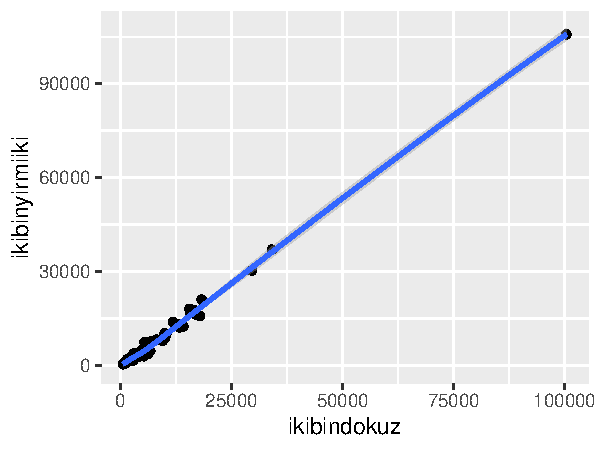
\includegraphics{final_files/figure-latex/plot-1} 

}

\caption{Son 4 yıl arasındaki değerleri gösteren girafik}\label{fig:plot-1}
\end{figure}
\begin{figure}

{\centering 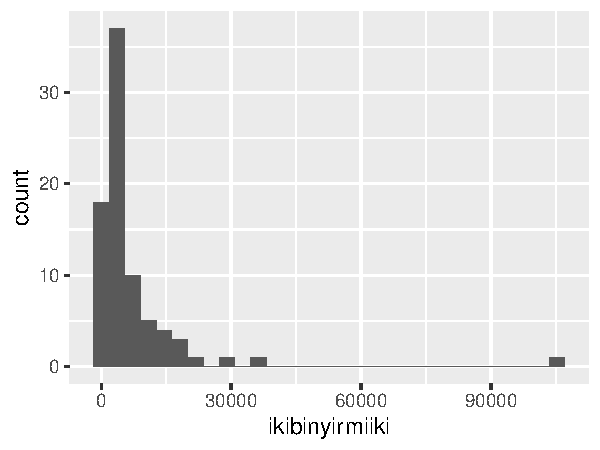
\includegraphics{final_files/figure-latex/plot-2} 

}

\caption{Son 4 yıl arasındaki değerleri gösteren girafik}\label{fig:plot-2}
\end{figure}

\hypertarget{sonuuxe7}{%
\section{Sonuç}\label{sonuuxe7}}

Veri setimizi incelediğimizde karşılaştığımız tablo ülkemizin büyük şehirlerinde artan nüfusa oranla evlenme sayılarının giderek düştüğü aşikâr bir gerçektir. Her ne kadar ülkemizin doğu kesiminde fazla bir azalmanın görülmese bile ilerleyen dönemlerden kırsaldan kente olan göçlerle birlikte o bölgede evlenme yaşının artacağı evlenme sayılarının azalacağı şekillinde bir öngörüde bulunabiliriz. Bununla birlikte azalan doğurganlığın ülkemiz nüfus açısından bir tehlike oluşturabilir. Bölgelerimizde İklim şartları, ailelerin yaşam tarzları ve geleneklerde şehirlere göre evlenme sayılarındaki değişkenliği açıklaya bilir. Aile yapısın bozulması da kuvvetli bağların bozulup kültürümüzün yok olmasına da sebep olabilmektedir. Bu sorunun çözümü kişilerin bilinçlendirilmesiyle ve devlet teşviğiyle mümkün kıllanabilir. Devletimiz değişen sosyal hayat şartları ve ekonomik problemlerin aşılmasında genç yaştaki en azından 24-30 yaş arasındaki bireylere desteğiyle mümkün kılınabilir. Bu problemin devlet eliyle çözülmesi daha mümkün gözükmektedir .Ancak bu gözlem verilerin bir müddet daha devam etmesi kesin sonuçlar elde etmemize yarar.

\newpage

\hypertarget{references}{%
\section{Kaynakça}\label{references}}

\hypertarget{refs}{}
\begin{CSLReferences}{1}{0}
\leavevmode\vadjust pre{\hypertarget{ref-bakanliugi2015turkiye}{}}%
BAKANLIĞI, A. V. S. P. ve MÜDÜRLÜĞÜ, A. V. T. H. G. (2015). T{Ü}RK{İ}YE'DE EVL{İ}L{İ}K TERC{İ}HLER{İ} N{İ}SAN 2015.

\leavevmode\vadjust pre{\hypertarget{ref-ccobanouglu2021turkiye}{}}%
Çobanoğlu, A. ve Serhat, T. (2021). T{ü}rkiye'de Yeniden Evlenme Olgusu: Cinsiyet ve Psikososyal De{ğ}i{ş}kenler Ba{ğ}lam{ı}nda Bir De{ğ}erlendirme. \emph{OPUS International Journal of Society Researches}, \emph{18}(44), 8092-8118.

\leavevmode\vadjust pre{\hypertarget{ref-ilhan2019marriage}{}}%
İlhan, S. T. ve Işık, Ş. (2019). The Marriage Life Experiences and Perceptions on The Early Years of The Marriage: Problems, Difficulties and Needs. \emph{Journal of Qualitative Research in Education}, \emph{7}(4).

\leavevmode\vadjust pre{\hypertarget{ref-kocc2017development}{}}%
KOÇ, B., TATLI, H. ve NAİMOĞLU, M. (2017). Development of Beekeeping in Bingol Province and Surveyable Beekeeping Possibilities. \emph{Proceeding Book}.

\end{CSLReferences}

\end{document}
